% Full instructions available at:
% https://github.com/elauksap/focus-beamertheme

\documentclass{beamer}
\usetheme[numbering=progressbar]{focus}
\usepackage{tikz}
\usetikzlibrary{positioning}
\usetikzlibrary{shapes,arrows}
\usepackage{transparent}
\usepackage{fancyvrb}
\usepackage{listings}
\definecolor{main}{RGB}{47, 161, 219}
%\definecolor{textcolor}{RGB}{128, 128, 128}
\definecolor{background}{RGB}{240, 247, 255}
\definecolor{textcolor}{RGB}{85, 87, 83}
\title{D4 Project}
\subtitle{PIBS - Passive Identification of BackScatter}
\author{TEAM CIRCL}
\titlegraphic{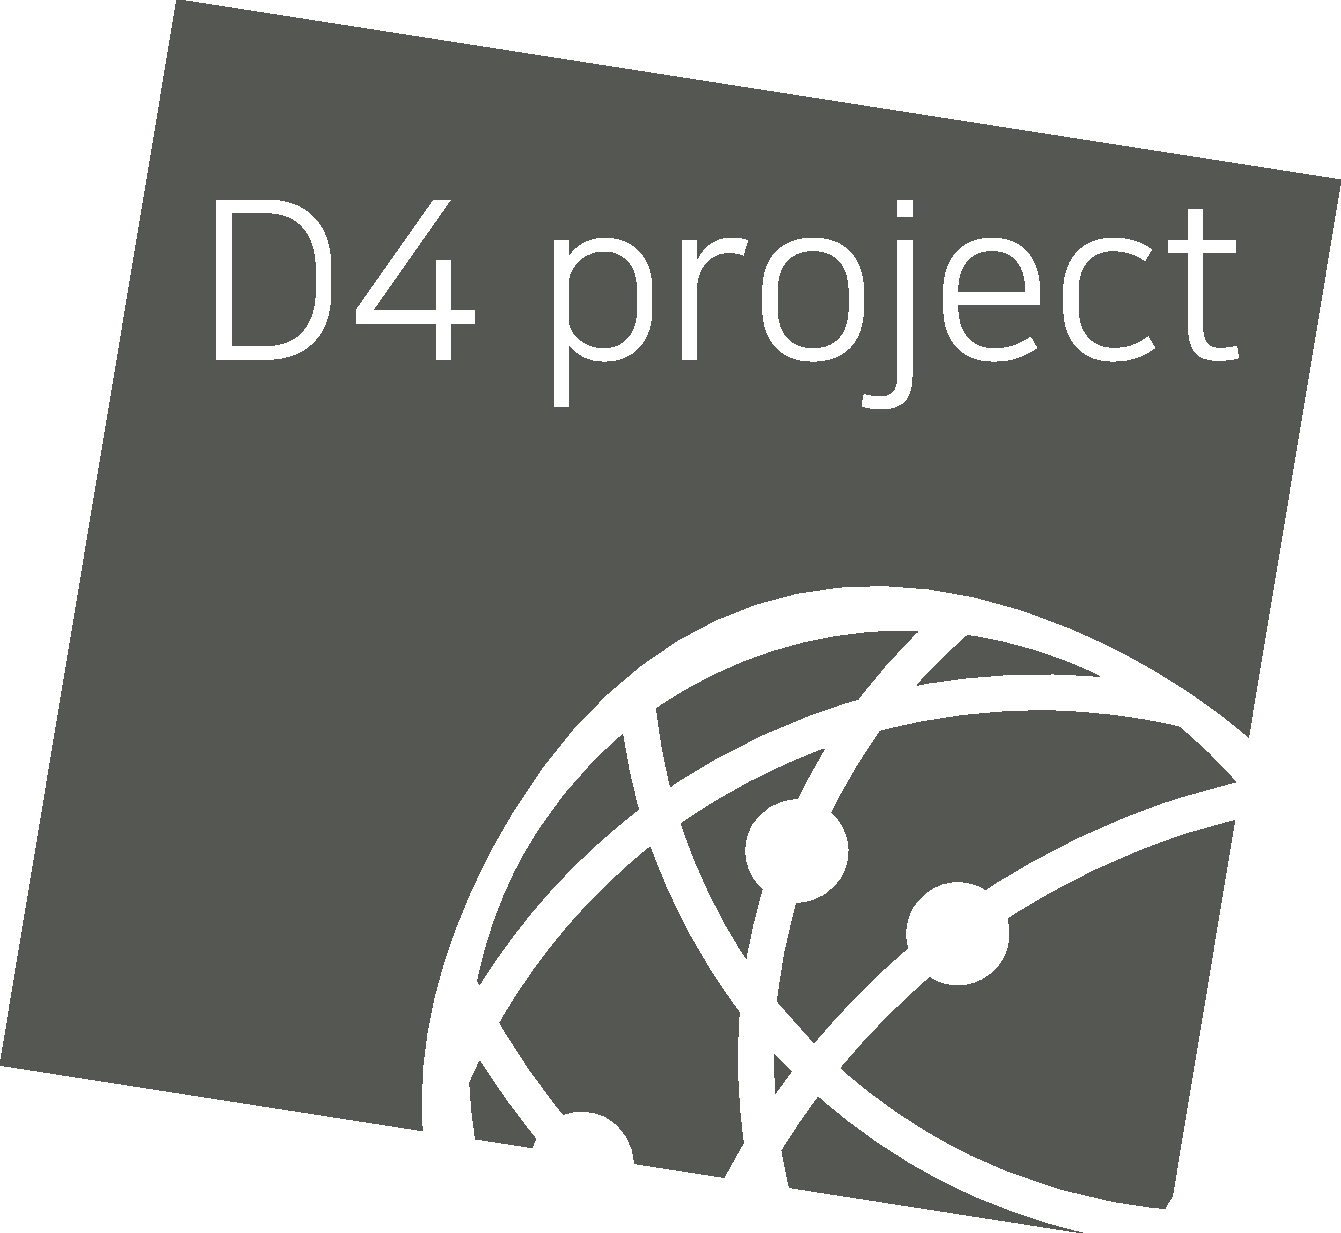
\includegraphics[scale=0.20]{d4-logo.pdf}}
\institute{Team CIRCL \\ \url{https://www.d4-project.org/}}
\date{20190329}

\begin{document}
    \begin{frame}
        \maketitle
    \end{frame}


\begin{frame}
    \frametitle{Open problems}
    \framesubtitle{Filter out potential backscatter traffic}
    \begin{itemize}
        \item Differentiate Scanning activities\footnote{\url{https://nmap.org/book/man-port-scanning-techniques.html}}
        \begin{itemize}
            \item TCP SYN scan
            \item XMAS scans
            \item ACK scans
            \item TCP Window scan
            \item TCP Maimon scan
            \item Custom TCP scan
        \end{itemize}
        \item Misconfigured systems
        \item Malicious packets against D4 infrastructure
	\item Handling file rotations
	\item Expiration of state tables
    \end{itemize}
\end{frame}

\end{document}
